\chapter{Speaker Identification e Verification}
\label{ch:speakerID}

\section{Descrizione del problema}
Nel contesto dell'analisi intelligente dei segnali sappiamo che lavorando con sorgenti audio
vorremmo avere una rappresentazione alternativa per ogni specifico segnale audio, chiamata appunto come
rappresentazione di \textbf{features}, che possiamo usare per task diversi. \\
Uno dei task che da sempre è studio di lavori (sia per la sua applicabilità pratica nel settore industriale, che
da un punto di vista di ricerca) è quello dello \text{Speaker Identification}. Infatti questo task trova grande interesse nei sistemi
di riconoscimento biometrici, diventando quindi un punto cruciale nel settore della sicurezza informatica. In generale, i sistemi biometrici
si basano sulle caratteristiche \textit{individuali e altamente discriminative} delle persone, presentando già il principale compito dei sistemi di riconoscimento: identificare
le persone correttamente e riconoscere se ci sono degli impostori, sulla base delle caratteristiche (o \textit{features}) di ogni singolo speaker. \\
Nel task della \textit{speaker identification}, il nostro obiettivo principale è cercare di estrarre dagli human speech di ogni singolo speaker una rappresentazione alternativa utile a rappresentare univocamente un soggetto, quindi costruire \textbf{speaker models}, che permettano
poi di riconoscere i singoli utenti tramite una classificaione o pattern-matching in generale. Lo scopo dello \textit{speaker models} è quello 
alla fine di creare un database di persone che conosco, al fine di avere abbastanza informazioni per poter riconoscere quel determinato speaker in seguito. 
Uno schema di funzionamento è riportato in \ref{fig:speakerschema} Il sistema viene diviso in due fasi:
\begin{itemize}
    \item una fase di training, o anche definita come \textit{enrolment}, dove acquisiamo audio da cui estrarre features da cui estrarre un database di speaker models
    \item Una fase di testing, dove andiamo a valutare quanti speaker riusciamo correttamente a riconoscere 
\end{itemize}

Quando però realizziamo la fase di testing dobbiamo distinguere tra una identificazione \textit{closed-set}, ovvero abbiamo un insieme di identità
che conosciamo e dobbiamo distinguere gli uni dagli altri, che una identificazione \textit{open-set}, dove invece dobbiamo identificare tra identità che conosciamo 
e quelle che invece non conosciamo e classifichiamo come sconosciute. \\
In questo contesto si inserisce la \textit{speaker verification}. Partiamo da una base di identification (dove quindi abbiamo un database di identità conosciute), e cerchiamo
di capire se un un nuovo speaker fa parte del nostro insieme o no. In questo caso il focus non è tanto l'identificazione, ma tanto il rejection dell'utente nel caso in cui 
non sia chi dica di essere. Facendo un esempio banale, se un utente parla ad un sistema di riconoscimento e dice di essere qualcun'altro, il sistema deve essere in grado di
identificarlo correttamente (anche qui, closed-set o open-set) e di assegnargli una identità, eventualmente "bloccandolo" se troviamo che non è che dice di essere. Parliamo quindi in
questo caso di rejection e acceptance di un determinato speaker, per valutare correttamente il sistema, sulla base per esempio di uno score (compito di solito svolto dal BackEnd) \\

Inoltre, entrambi i task possono essere dipendenti o indipendenti dai vincoli lessicali \cite{tu2022survey}. Infatti distinguiamo tra \textit{Text-Indipendent} e \textit{Text-Dipendent},
sia in ottica Speaker Identification che Verification. Per vincolo lessicale intendiamo infatti che lo speaker deve dire una determinata sequenza di parole, che in pratica
corrisponde a pronunciare una \textit{keyword o passphrase}.

\begin{figure}[ht]
    \centering
    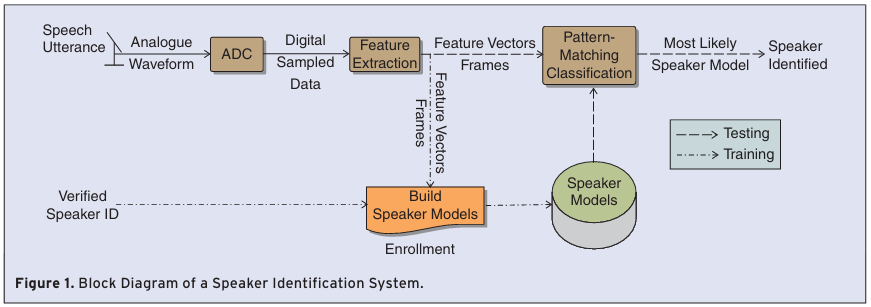
\includegraphics[width=1.0\textwidth]{./ch1/speaker_id.png}
    \caption{Sistema di Speaker identification, \protect\cite{togneri2011overview}}
    \label{fig:speakerschema}
\end{figure}


\begin{figure}[ht]
    \centering
    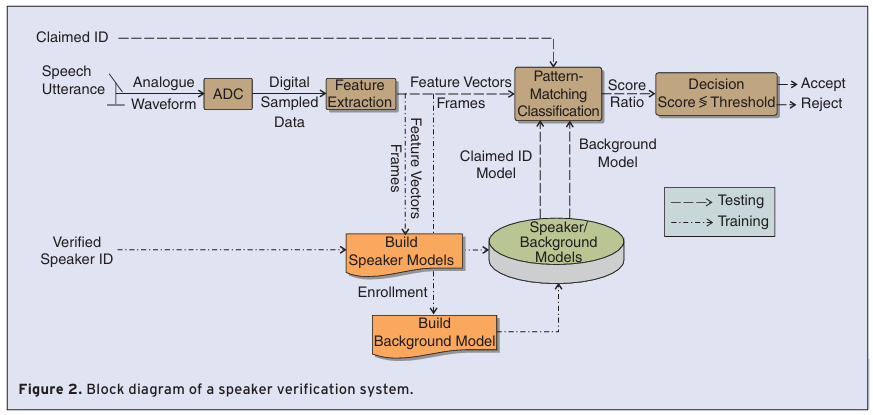
\includegraphics[width=1.0\textwidth]{./ch1/speaker_ver.png}
    \caption{Sistema di Speaker Verification, \protect\cite{togneri2011overview}}
    \label{fig:speakerschemaver}
\end{figure}

\section{Valutazione dei sistemi: metriche e metodologie}
Per poter correttamente valutare un sistema di identificazione e verifica delle identità dobbiamo basarci su specifiche metriche e metodologie.
Per quanto riguarda le metodologie, sia in open-set che closed-set, partiamo da un training set composto da segnali audio a cui applichiamo la classica analisi,
al fine di poter effettuare operazioni di estrazione di features. Training e Testing sono composti da audio composto da speaker noti nel caso di speaker identification, da speaker diversi nel caso di speaker verification.
Per quanto riguarda le metriche da utilizzare, queste sono diverse a seconda del task. Nel task della identificazione è importante capire quanti utenti riusciamo a riconoscere
e distinguere correttamente, quindi valutare metriche come la \textit{precisione, la accuracy, la f1score} per ogni speaker e in maniera complessiva del sistema. 

Per quanto riguarda invece la verifica delle identità è più importante riconoscere quante persone riusciamo correttamente a riconoscere come intrusi e quindi bloccare e non far accedere al sistema. 
Quindi questo task è da vedere più come classificazione binaria che multiclasse, perché a noi interessano \textit{True Positive Rate (quante persone riusciamo correttamente a far passare)} e \textit{False Positive Rate (quante persone facciamo passare sebbene siano impostori)}.
Una metrica aggregata è la \textbf{Equal Error Rate (EER)}, metrica comune nei sistemi biometrici. Si riferisce al punto in cui il tasso di falsi accettamenti (\textbf{(FAR - False Acceptance Rate}) è uguale al tasso di falsi rifiuti (\textbf{FRR - False Rejection Rate}). 
In termini di TPR e TNR, la FAR è il complementare del TNR (percentuale di impostori correttamente identificati), quindi coincide con la FPR, mentre la TPR è il complementare della FRR (percentuale di parlanti autentici e correttamente accettati).
Un riassunto è riportato in Tab.\ref{tab:metriche}

\begin{table}[ht]
    \centering
    \renewcommand{\arraystretch}{1.4}
    \begin{tabular}{@{} m{4cm} m{5.5cm} m{6.5cm} @{}}
    \toprule
    \textbf{Task} & \textbf{Obiettivo} & \textbf{Metriche utilizzate} \\
    \midrule
    \textbf{Speaker Identification} (Closed-set) & 
    Riconoscere l'identità del parlante tra un insieme noto di speaker (classificazione multiclasse). & 
    \begin{itemize}
    \item Accuracy
    \item Precision, Recall, F1-score (per classe e macro media)
    \item Confusion Matrix
    \end{itemize} \\
    \midrule
    \textbf{Speaker Verification} (Open-set) & 
    Verificare se un parlante è chi dichiara di essere (classificazione binaria: accetta/rifiuta). & 
    \begin{itemize}
    \item True Positive Rate (TPR)
    \item False Positive Rate (FPR)
    \item False Acceptance Rate (FAR)
    \item False Rejection Rate (FRR)
    \item Equal Error Rate (EER)
    \item ROC / DET Curve
    \end{itemize} \\

    \bottomrule
    \end{tabular}
    \caption{Task, obiettivi e metriche nei sistemi di speaker recognition}
    \label{tab:metriche}
\end{table}

\section{Scenari applicativi}
Come detto prima, questi task si concentrano sopratutto nell'ottica di sistemi di riconoscimento biometrici, con particolare
focus sia al riconoscimento che alla verifica dell'identità. ques'ultimo aspetto diventa chiave e cruciale per i ssitemi di sicurezza 
basati su riconoscimento della voce (biometria dinamica), per il controllo degli accessi o ulteriore fattore di autenticazione. \\
Lo scopo di questo progetto è quello di esplorare entrambi gli aspetti, con particolare focus alle tecniche principali che permettono di identificare
gli speaker con metodologie basate sul Deep Learning, esplorando anche come un sistema di identificazione può essere traslato ed adattato
in un sistema di verifica delle identità tramite classificazione binaria \textit{one-vs-others}, dove i nostri utenti VERI sono quelli del nostro dataset,
quelli invece FALSI sono quelli che non fanno parte del dataset. 